%!TEX program = pdflatex
\documentclass[a4paper,conference]{IEEEtran}

\usepackage{ifluatex}
\ifluatex
  \usepackage{fontspec}
  \usepackage{polyglossia} % babel replacement for use with fontspec
  \setdefaultlanguage[variant=american]{english}
  \selectlanguage[variant=american]{english}
\else
  \usepackage[utf8]{inputenc}
  \usepackage[T1]{fontenc}
  \usepackage[american]{babel}
  \usepackage{textcomp}
  %\DeclareUnicodeCharacter{20AC}{\euro{}}
  %\usepackage{eurosym}
\fi

\usepackage[acronym, nomain, nowarn]{glossaries}
\loadglsentries{acronyms}
\usepackage[hyphens]{url}
%\usepackage[pdfhighlight=/O, hidelinks, unicode=true]{hyperref}
\usepackage{mathtools}
\usepackage{fixmath}
\usepackage{algorithm2e}
%\usepackage{subcaption}
\usepackage{siunitx}
%\DeclareSIUnit{\EUR}{\text{\texteuro}} % gulps up subsequent symbols, commented out
\DeclareSIUnit\year{yrs}
\sisetup{load-configurations = abbreviations,binary-units, per-mode=symbol}
\usepackage{csquotes}
\usepackage{booktabs}
\usepackage{tabu}
\usepackage{rotating}
\makeglossaries
\usepackage[url=false,doi=false,backend=biber,style=ieee,isbn=false,sorting=none,minnames=1,maxnames=2]{biblatex}
\addbibresource{literature.bib}
\usepackage[inline]{enumitem}

\usepackage[np]{numprint}
\npstyleenglish

\usepackage[bordercolor=white]{todonotes}
\usepackage{balance}


\usepackage{cleveref}
\crefformat{footnote}{#2\footnotemark[#1]#3}


\begin{document}

% \title{End-to-End Lag is Complicated: A Detailed Model for ``Overwatch''}
%\title{It's Complicated: An End-to-End Lag Model for the Multiplayer Shooter Overwatch}
\title{Exploring the Transmission Behaviour of Overwatch: The Source of Lag}

\author{
\IEEEauthorblockN{Florian Metzger}
\IEEEauthorblockA{Chair of Communication Networks\\
University of Würzburg, Germany\\
\texttt{florian.metzger@uni-wuerzburg.de}}
\and
\IEEEauthorblockN{Roman Heger}
%\IEEEauthorblockA{Chair of Modeling of Adaptive Systems\\
University of Duisburg-Essen, Germany\\
%\texttt{florian.metzger@uni-due.de}}
}


\maketitle

% TODO: - the introduction is fragmentary and badly written;

% TODO: Perform proof-reading of the paper to correct minor spelling/grammar mistakes and (as stated in the previous part of the review) provide more details on distributions for readers with less mathematical knowledge. Minor improvements regarding readability of the paper, especially mathematical background, would be to provide either references or some overview information on distributions(Gamma, Normal,Cauchy).

% TODO: - Investigate auto-correlation and influence factors (additional delay, packet loss, smaller time-scales) on the lag.

% TODO: - The paper does the implicit assumption that the lag can be models as independent processes and there is no investigation of correlations/auto-correlation on smaller time scales. 
% TODO: - There is only one network configuration evaluated. Additional delay in the network or packet loss may also change the sending behavior of the client and/or server.
% TODO: - It is unclear how the models can be generalized. The measurements cover only one set of parameters.

% TODO: Proofread the paper, there are some minor punctuation issues and some double words and more. You should also consider to consult a native english speaker and let him rephrase the "worst" parts -> there is a lot of german grammar ... 

% TODO: I don't see any major weakness in this paper. It would be good to elaborate more on the investigation to help unfamiliar readers to understand the overall approach. Moreover, some background and related work would helpful to highlight the scientific contribution. However, this would very likely exceed the page limit.

% TODO: - The proposed methodology and model, as pointed out by the same Authors, is highly specific to the kind of game and to the deployment scenario (e.g., characteristics and resource availability at the player's PC). Which generality? Possibility to apply to different deployment scenarios? How?
% TODO: - There are no quantitative results showing that the proposed modeling is well fitting the experimental results about lag that can be directly measured in in-the-field experimentation. How to validate in-the-field the proposed model?

%!TEX root = paper.tex
%%%%%%%%%%%%%%%%%%%%%%%%%%%%%%%%%%%%%%%%%%%%%%%%%%%%%%%%%%%%%%%%%%%%%%%%%%%%%%%

\newglossaryentry{cg}{name={cloud gaming},description={Gaming in the cloud}}
\newglossaryentry{cr}{name={cloud rendering},description={In contrast to \gls{Gaas}, the game is provided by the customer and is only rendered in the cloud}}

%\newacronym[description={\glslink{2g}{Second Generation}}]{2G}{2G}{Second Generation}
\newacronym{2G}{2G}{Second Generation}
\newacronym{3G}{3G}{Third Generation}
\newacronym{3GPP}{3GPP}{Third Generation Partnership Project}
\newacronym{AAA}{AAA}{Authentication, Authorization and Accounting}
\newacronym{AAC}{AAC}{Advanced Audio Coding}
\newacronym{ABI}{ABI}{Application Binary Interface}
\newacronym{AMBR}{AMBR}{Aggregate Maximum Bit-Rate}
\newacronym{ANOVA}{ANOVA}{Analysis of Variance}
\newacronym{API}{API}{Application Programming Interface}
\newacronym{APM}{APM}{Actions per Minute}
\newacronym{APN}{APN}{Access Point Name}
\newacronym{AQM}{AQM}{Active Queue Management}
\newacronym{ARQ}{ARQ}{Automatic Repeat Request}
\newacronym{ASN.1}{ASN.1}{Abstract Syntax Notation One}
\newacronym{ATM}{ATM}{Asynchronous Transfer Mode}
\newacronym{AU}{AU}{Access Unit}
\newacronym{AuC}{AuC}{Authentication Centre}
\newacronym{AVC}{AVC}{Advanced Video Coding}
\newacronym{BDP}{BDP}{Bandwidth-Delay Product}
\newacronym{BGP}{BGP}{Border Gateway Protocol}
\newacronym{BMC}{BMC}{Broadcast/Multicast Control}
\newacronym{BSC}{BSC}{Base Station Controller}
\newacronym{BSD}{BSD}{Berkeley Software Distribution}
\newacronym{BSS}{BSS}{Base Station Subsystem}
\newacronym{BTS}{BTS}{Base Transceiver Station}
\newacronym{CAMEL}{CAMEL}{Customised Applications for Mobile Networks Enhanced Logic}
\newacronym{CAPEX}{CAPEX}{CAPital EXpenditure}
\newacronym{CCG}{CCG}{Collectible Card Game}
\newacronym{CDF}{CDF}{Cumulative Distribution Function}
\newacronym{CDN}{CDN}{Content Distribution Network}
\newacronym{CDMA}{CDMA}{Code Division Multiple Access}
\newacronym{CELLDCH}{CELL\_DCH}{Dedicated Channel}
\newacronym{CELLFACH}{CELL\_FACH}{Forward Access Channel}
\newacronym{CELLPCH}{CELL\_PCH}{Cell Paging Channel}
\newacronym{CGN}{CGN}{Carrier-grade \acrshort{NAT}}
\newacronym{CI}{CI}{Continuity Index}
\newacronym{CN}{CN}{Core Network}
\newacronym{CPU}{CPU}{Central Processing Unit}
\newacronym{CS}{CS}{Circuit Switching}
\newacronym{CSG}{CSG}{Closed Subscriber Group}
\newacronym{CSS}{CSS}{Cascading Style Sheets}
\newacronym{DANE}{DANE}{DNS-Based Authentication of Named Entities}
\newacronym{DASH}{DASH}{Dynamic Adaptive Streaming over \acrshort{HTTP}}
\newacronym{DCCP}{DCCP}{Datagram Congestion Control Protocol}
\newacronym{DCE}{DCE}{Direct Code Execution}
\newacronym{DDoS}{DDoS}{Distributed \acrshort{DoS}}
\newacronym{DES}{DES}{Discrete Event Simulation}
\newacronym{DF}{DF}{Delay Factor}
\newacronym{DLEP}{DLEP}{Dynamic Link Exchange Protocol}
\newacronym{DLNA}{DLNA}{Digital Living Network Alliance}
\newacronym{DNS}{DNS}{Domain Name System}
\newacronym{DNSSEC}{DNSSEC}{\acrshort{DNS} Security Extensions}
\newacronym{DOCSIS}{DOCSIS}{Data Over Cable Service Interface Specification}
\newacronym{DoS}{DoS}{Denial of Service}
\newacronym{DPI}{DPI}{Deep Packet Inspection}
\newacronym{DRM}{DRM}{Digital Rights Management}
\newacronym{DSL}{DSL}{Digital Subscriber Line}
\newacronym{DTLS}{DTLS}{Datagram \acrshort{TLS}}
\newacronym{DTN}{DTN}{Delay-Tolerant Networking}
\newacronym{E2E}{E2E}{end-to-end}
\newacronym{ECDF}{ECDF}{Empirical \acrshort{CDF}}
\newacronym{ECM}{ECM}{EPS Connection Management}
\newacronym{ECN}{ECN}{Explicit Congestion Notification}
\newacronym{EDGE}{EDGE}{Enhanced Data Rates for \acrshort{GSM} Evolution}
\newacronym{EEG}{EEG}{Electroencephalography}
\newacronym{EIR}{EIR}{Equipment Identity Register}
\newacronym{EMM}{EMM}{Evolved Mobility Management}
\newacronym{eNB}{eNB}{Evolved Node B}
\newacronym{EPC}{EPC}{Evolved Packet Core}
\newacronym{EPS}{EPS}{Evolved Packet System}
\newacronym{ES}{ES}{Elementary Stream}
\newacronym{ETSI}{ETSI}{European Telecommunications Standards Institute}
\newacronym{E-UTRAN}{E-UTRAN}{Evolved \acrshort{UTRAN}}
\newacronym{FEC}{FEC}{Forward Error Correction}
\newacronym{fEMG}{fEMG}{Facial Electromyography}
\newacronym{FPS}{FPS}{First-Person Shooter}
\newacronym{FOSS}{FOSS}{Free and open-source software}
\newacronym{FSM}{FSM}{finite-state machine}
\newacronym{FTW}{FTW}{Telecommunications Research Center Vienna}
\newacronym{GaaS}{GaaS}{Gaming as a Service} %description={The game is provided by the platform operator and is rendered in the cloud}}
\newacronym{GERAN}{GERAN}{\acrshort{GSM}/\acrshort{EDGE} Radio Access Network}
\newacronym{GGSN}{GGSN}{Gateway \acrshort{GPRS} Support Node}
\newacronym{GMSC}{GMSC}{Gateway \acrshort{MSC}}
\newacronym{GPL}{GPL}{GNU General Public License}
\newacronym{GPLv3}{GPLv3}{\acrshort{GPL} version 3}
\newacronym{GPRS}{GPRS}{General Packet Radio System}
\newacronym{GPS}{GPS}{Global Positioning System}
\newacronym{GSM}{GSM}{Global System for Mobile Communications}
\newacronym{GSMA}{GSMA}{\acrshort{GSM} Association}
\newacronym{gtp}{GTP}{GPRS Tunneling Protocol}
\newacronym{GTP-C}{GTP-C}{\acrshort{gtp} Control}
\newacronym{GTP-U}{GTP-U}{\acrshort{gtp} User}
\newacronym{gtpv2}{GTPv2}{\acrshort{gtp} version 2}
\newacronym{GPU}{GPU}{Graphics Processing Unit}
\newacronym{GUI}{GUI}{Graphical User Interface}
\newacronym{HLR}{HLR}{Home Location Register}
\newacronym{HLS}{HLS}{HTTP Live Streaming}
\newacronym{HOL}{HOL}{Head-of-line}
\newacronym{HSDPA}{HSDPA}{High-Speed Downlink Packet Access}
\newacronym{HSPA}{HSPA}{High Speed Packet Access}
\newacronym{HSPA+}{HSPA+}{High Speed Packet Access Plus}
\newacronym{HSS}{HSS}{Home Subscriber Server}
\newacronym{HSUPA}{HSUPA}{High Speed Uplink Packet Access}
\newacronym{HTML}{HTML}{HyperText Markup Language}
\newacronym{HTTP}{HTTP}{HyperText Transfer Protocol}
\newacronym{HTTPS}{HTTPS}{\acrshort{HTTP} Secure}
\newacronym{IAB}{IAB}{Internet Architecture Board}
\newacronym{IAT}{IAT}{Inter Arrival Time}
\newacronym{ICE}{ICE}{Interactive Connectivity Establishment}
\newacronym{ICMP}{ICMP}{Internet Control Message Protocol}
\newacronym{IE}{IE}{Information Element}
\newacronym{IEC}{IEC}{International Electrotechnical Commission}
\newacronym{IEEE}{IEEE}{Institute of Electrical and Electronics Engineers}
\newacronym{IETF}{IETF}{Internet Engineering Task Force}
\newacronym{IGMP}{IGMP}{Internet Group Management Protocol}
\newacronym{IMAP}{IMAP}{Internet Message Access Protocol}
\newacronym{IMAPS}{IMAPS}{\acrshort{IMAP} Secure}
\newacronym{IMEI}{IMEI}{International Mobile Equipment Identity}
\newacronym{IMS}{IMS}{IP Multimedia Subsystem}
\newacronym{IMSI}{IMSI}{International Mobile Subscriber Identity}
\newacronym{IoE}{IoE}{Internet of Everything}
\newacronym{IoT}{IoT}{Internet of Things}
\newacronym{IP}{IP}{Internet Protocol}
\newacronym{IPC}{IPC}{Inter-Process Communication}
\newacronym{IPv4}{IPv4}{\acrshort{IP} version 4}
\newacronym{IPv6}{IPv6}{\acrshort{IP} version 6}
\newacronym{IPTV}{IPTV}{Internet Protocol television}
\newacronym{ISDN}{ISDN}{Integrated Services Digital Network}
\newacronym{ISO}{ISO}{International Organization for Standardization}
\newacronym{ISOC}{ISOC}{Internet Society}
\newacronym{ISP}{ISP}{Internet Service Provider}
\newacronym{ITU}{ITU}{International Telecommunication Union}
\newacronym{ITU-T}{ITU-T}{\acrshort{ITU} Telecommunication Standardization Sector}
\newacronym{JSON}{JSON}{JavaScript Object Notation}
\newacronym{KISS}{KISS}{``Keep it simple, stupid''}
\newacronym{LAN}{LAN}{Local Area Network}
\newacronym{LEDBAT}{LEDBAT}{Low Extra Delay Background Transport}
\newacronym{LGPLv3}{LGPLv3}{GNU Lesser General Public License version 3}
\newacronym{LISP}{LISP}{Locator/Identifier Separation Protocol}
\newacronym{LTE}{LTE}{Long Term Evolution}
\newacronym{M2M}{M2M}{Machine-to-Machine}
\newacronym{MAC}{MAC}{Media Access Control}
\newacronym{MANET}{MANET}{Mobile Ad Hoc Network}
\newacronym{MAP}{MAP}{Mobile Application Part}
\newacronym{MBMS}{MBMS}{Multimedia Broadcast Multicast Services}
\newacronym{MBR}{MBR}{Maximum Bitrate}
\newacronym{MDI}{MDI}{Media Delivery Index}
\newacronym{METAWIN}{METAWIN}{Measurement and Traffic Analysis in Wireless Networks}
\newacronym{MGW}{MGW}{Media Gateway}
\newacronym{MIME}{MIME}{Multipurpose Internet Mail Extensions}
\newacronym{MM}{MM}{Mobility Management}
\newacronym{MME}{MME}{Mobility Management Entity}
\newacronym{MMO}{MMO}{Massively Multiplayer Online}
\newacronym{MMS}{MMS}{Microsoft Media Server}
\newacronym{MOS}{MOS}{Mean Opinion Score}
\newacronym{MS}{MS}{Mobile Station}
\newacronym{MS-ID}{MS-ID}{Mobile Station Identifier}
\newacronym{MSC}{MSC}{Mobile Switching Center}
\newacronym{MSISDN}{MSISDN}{Mobile Subscriber Integrated Services Digital Network-Number}
\newacronym{MSE}{MSE}{Mean Squared Error}
\newacronym{MTC}{MTC}{Machine-Type Communications}
\newacronym{MTU}{MTU}{Maximum Transmission Unit}
\newacronym{NAS}{NAS}{Network-Attached Storage}
\newacronym{NAT}{NAT}{Network Address Translation}
\newacronym{NBAP}{NBAP}{Node B Application Part}
\newacronym{NFC}{NFC}{Near Field Communication}
\newacronym{NFV}{NFV}{Network Function Virtualization}
\newacronym{NSAPI}{NSAPI}{Network Service Access Point Identifier}
\newacronym{NSC}{NSC}{Network Simulation Cradle}
\newacronym{O3GM}{O3GM}{Open3G Map}
\newacronym{OMC}{OMC}{Operation and Maintenance Centre}
\newacronym{OPEX}{OPEX}{OPerational EXpenditure}
\newacronym{os}{OS}{Operating System}
\newacronym{OSI}{OSI}{Open Systems Interconnection}
\newacronym{OSPF}{OSPF}{Open Shortest Path First}
\newacronym{P2P}{P2P}{Peer-to-Peer}
\newacronym{PAN}{PAN}{Personal Area Network}
\newacronym{PC}{PC}{Personal Computer}
\newacronym{PCC}{PCC}{Policy and Charging Control}
\newacronym{PCO}{PCO}{Protocol Configuration Options}
\newacronym{PCEF}{PCEF}{Policy and Charging Enforcement Function}
\newacronym{PCRF}{PCRF}{Policy and Charging Rules Function}
\newacronym{PDCP}{PDCP}{Packet Data Convergence Protocol}
\newacronym{PDN}{PDN}{Public Data Network}
\newacronym{PDP}{PDP}{Packet Data Protocol}
\newacronym{PEVQ}{PEVQ}{Perceptual Evaluation of Video Quality}
\newacronym{PGW}{PGW}{Packet Gateway}
\newacronym{PI}{PI}{Pause Intensity}
\newacronym{PLMN}{PLMN}{Public Land Mobile Network}
\newacronym{PMIPv6}{PMIPv6}{Proxy Mobile \acrshort{IPv6}}
\newacronym{PMTU}{PMTU}{Path \acrshort{MTU}}
\newacronym{PON}{PON}{Passive Optical Network}
\newacronym{PPPoE}{PPPoE}{Point-to-Point Protocol over Ethernet}
\newacronym{PRNG}{PRNG}{Pseudorandom Number Generator}
\newacronym{PS}{PS}{Packet Switching}
\newacronym{PSNR}{PSNR}{Peak Signal-to-Noise Ratio}
\newacronym{QoE}{QoE}{Quality of Experience}
\newacronym{QoS}{QoS}{Quality of Service}
\newacronym{QUIC}{QUIC}{Quick UDP Internet Connections}
\newacronym{RAB}{RAB}{Radio Access Bearer}
\newacronym{RAN}{RAN}{Radio Access Network}
\newacronym{RANAP}{RANAP}{Radio Access Network Application Part}
\newacronym{RAI}{RAI}{Routeing Area Identity}
\newacronym{RBI}{RBI}{Reporting Body Identifier}
\newacronym{RAT}{RAT}{Radio Access Technology}
\newacronym{REST}{REST}{Representational State Transfer}
\newacronym{RFC}{RFC}{Request for Comments}
\newacronym{RIP}{RIP}{Routing Information Protocol}
\newacronym{RLC}{RLC}{Radio Link Control}
\newacronym{RNC}{RNC}{Radio Network Controller}
\newacronym{RPC}{RPC}{Remote Procedure Call}
\newacronym{RPG}{RPG}{Role-Playing Game}
\newacronym{RRC}{RRC}{Radio Resource Control}
\newacronym{RSS}{RSS}{Rich Site Summary}
\newacronym{rtcp}{RTCP}{\acrshort{rtp} Control Protocol}
\newacronym{RTMP}{RTMP}{Real Time Messaging Protocol}
\newacronym{rtp}{RTP}{Real-time Transport Protocol}
\newacronym{RTS}{RTS}{Real-time Strategy game}
\newacronym{RTSP}{RTSP}{Real Time Streaming Protocol}
\newacronym{RTT}{RTT}{Round-Trip Time}
\newacronym{RV}{RV}{Random Variable}
\newacronym{S1AP}{S1AP}{S1 Application Protocol}
\newacronym{SAE}{SAE}{System Architecture Evolution}
\newacronym{SAP}{SAP}{Session Announcement Protocol}
\newacronym{osiSAP}{SAP}{Service Access Point}
\newacronym{SCCP}{SCCP}{Signalling Connection Control Part}
\newacronym{SCTP}{SCTP}{Stream Control Transmission Protocol}
\newacronym{SDN}{SDN}{Software Defined Networking}
\newacronym{SMTP}{SMTP}{Simple Mail Transfer Protocol}
\newacronym{SMTPS}{SMTPS}{\acrshort{SMTP} Secure}
\newacronym{SDP}{SDP}{Session Description Protocol}
\newacronym{SDR}{SDR}{Software Defined Radio}
\newacronym{SGSN}{SGSN}{Serving \acrshort{GPRS} Support Node}
\newacronym{SGW}{SGW}{Serving Gateway}
\newacronym{SIM}{SIM}{Subscriber Identity Module}
\newacronym{SIP}{SIP}{Session Initiation Protocol}
\newacronym{SQL}{SQL}{Structured Query Language}
\newacronym{SS7}{SS7}{Signalling System No. 7}
\newacronym{SSD}{SSD}{Solid State Disk}
\newacronym{SSIM}{SSIM}{Structural SIMilarity}
\newacronym{STUN}{STUN}{Session Traversal Utilities for \acrshort{NAT}}
\newacronym{SV}{SV}{Software Version}
\newacronym{SVC}{SVC}{Scalable Video Coding}
\newacronym{POTS}{POTS}{Plain Old Telephone Service}
\newacronym{PSTN}{PSTN}{Public Switched Telephone Network}
\newacronym{TAC}{TAC}{Type Allocation Code}
\newacronym{TCAP}{TCAP}{Transaction Capabilities Application Part}
\newacronym{TCP}{TCP}{Transmission Control Protocol}
\newacronym{TEID}{TEID}{Tunnel Endpoint Identifier}
\newacronym{TFT}{TFT}{Traffic Flow Template}
\newacronym{TLS}{TLS}{Transport Layer Security}
\newacronym{TS}{TS}{Technical Specification}
\newacronym{TTI}{TTI}{Transmission Time Interval}
\newacronym{UDP}{UDP}{User Datagram Protocol}
\newacronym{UE}{UE}{User Equipment}
\newacronym{UMTS}{UMTS}{Universal Mobile Telecommunications System}
\newacronym{UPnP}{UPnP}{Universal Plug and Play}
\newacronym{URA}{URA}{\acrshort{UTRAN} Registration Area}
\newacronym{URAPCH}{URA\_PCH}{\acrshort{URA} Paging Channel}
\newacronym{URL}{URL}{Uniform Resource Locator}
\newacronym{USIM}{USIM}{Universal Subscriber Identity Module}
\newacronym{uTP}{$\mu$TP}{Micro Transport Protocol}
\newacronym{UTRAN}{UTRAN}{\acrshort{UMTS} Terrestrial Radio Access Network}
\newacronym{VANET}{VANET}{Vehicular Ad Hoc Network}
\newacronym{VDSL}{VDSL}{Very-high-bit-rate Digital Subscriber Line}
\newacronym{VB}{VB}{Virtual Buffer}
\newacronym{VM}{VM}{Virtual Machine}
\newacronym{VMM}{VMM}{Virtual Machine Manager}
\newacronym{VoD}{VoD}{Video on Demand}
\newacronym{VoIP}{VoIP}{Voice over \acrshort{IP}}
\newacronym{VQEG}{VQEG}{Video Quality Experts Group}
\newacronym{W3C}{W3C}{World Wide Web Consortium}
\newacronym{WebRTC}{WebRTC}{Web Real-Time Communication}
\newacronym{WMSP}{WMSP}{Windows Media \acrshort{HTTP} Streaming Protocol}
\newacronym{XML}{XML}{Extensible Markup Language}
\newacronym{XMPP}{XMPP}{Extensible Messaging and Presence Protocol}

%!TEX root = paper.tex
%%%%%%%%%%%%%%%%%%%%%%%%%%%%%%%%%%%%%%%%%%%%%%%%%%%%%%%%%%%%%%%%%%%%%%%%%%%%%%%%
\begin{abstract}

This paper explores all the different factors in an online multiplayer game, namely Overwatch, that can contribute to the dreaded end-to-end lag, which has a direct impact on the subjective quality one experiences when playing video games. In its investigation, this paper reveals surprising effects in the game's networking behavior that are omitted when colloquially talking about, e.g. a \SI{60}{\hertz} update rate, but must be considered nonetheless. These insights, gained from examining network traces of Overwatch matches that were played on a realistic, resource constrained PC, can then be used to refine end-to-end lag simulation models and reach a better understanding of all responsible components.

\end{abstract}
%!TEX root = paper.tex
%%%%%%%%%%%%%%%%%%%%%%%%%%%%%%%%%%%%%%%%%%%%%%%%%%%%%%%%%%%%%%%%%%%%%%%%
%%%%%%%

\section{Introduction}

In theory, video games are simple: Retrieve an input, process it to update the game state, then display the results. But in praxis this gets a lot more complicated through the dynamic behavior of all involved factors. Especially when you add competitive multiplayer in to the mix and must synchronize the game states of the (authoritative) game server and each of the clients. Each of these components can then contribute to the \gls{E2E} lag, which will have an impact on each players' interactivity, and such on the perceived quality of the game as well\cite{Claypool:2006:LPA:1167838.1167860,7965676}. 

As to the extent of the impact of this lag on the perceived quality, many different factors can play a role, not just, as originally thought, the genre of the game in question \cite{mollertowards,Slivar:2016:CGQ:2910017.2910602}. In theory, the lag components of a video game can be measured \cite{7148095} or modeled in simulation \cite{Metzger+2016}. But in praxis the involved processes can get a lot more dynamic than stated in basic theory. 

The resource-constrained nature, where the video game can not maintain a stable frame rate, can play a major role. Most research in the past has assumed ideal conditions on this matter. Sufficient CPU and GPU resources to maintain, e.g., a frame rate of \SI{60}{\hertz}, as well as sufficient resources at the server to handle all all of the users' input events. Yet, in reality this is often not the case. 

% Anectdotally correct, but do we have any evidence, references on this?
% Or do we just argue that this is a common preference, as also targeted at by console manufactures/developers (aim for 30fps instead of something higher)
% Additionally: competitive players will often do the opposite to gain potential (and again, anectdotal) advantages. esp. e.g. observed in CSGO; advantages through both a better performance, but also through less visual complexity, less noise to distract
According to the Steam Hardware Survey\footnote{\url{https://store.steampowered.com/hwsurvey/}} The typical PC video game player tends not to have the latest or most powerful iteration of hardware components, but still wants to turn up the game's settings to enjoy a better graphical fidelity, often at the cost of frame rate. But this in turn affects all associated components relevant to the \gls{E2E} lag, including the command send rate from the game client to the server. Similar variations will occur at the server's side and impact the game state update transmission rates to the game clients.

This paper explores such a resource-constrained case and its effect on the popular team-based first-person shooter \textsc{Overwatch} on the PC. We recorded several game sessions and on this basis examine and model all lag-relevant components. These models are then used to refine the \gls{E2E} lag simulation of \cite{Metzger+2016}.

This work is a follow-up to the lag simulator presented in \cite{Metzger+2016} with a specific use case (Overwatch), in a specific environment (resource constrained), and thus with limited, and definitely not generalizable results.
And yet, those conditions are not particularly rare, and the ideal behavior is just that. Ideal, intended behavior in a scenario where everything works perfectly. Due to the variety in computer hardware and the fact that games often push the given hardware to their limits --- to produce good image quality at acceptable performance levels --- video games often run into resource limits. And 
%!TEX root = paper.tex
%%%%%%%%%%%%%%%%%%%%%%%%%%%%%%%%%%%%%%%%%%%%%%%%%%%%%%%%%%%%%%%%%%%%%%%%%%%%%%%%
\section{Examining Individual Lag Components}
\label{sec:lagmodel}

\begin{figure*}[t]
	\centering
	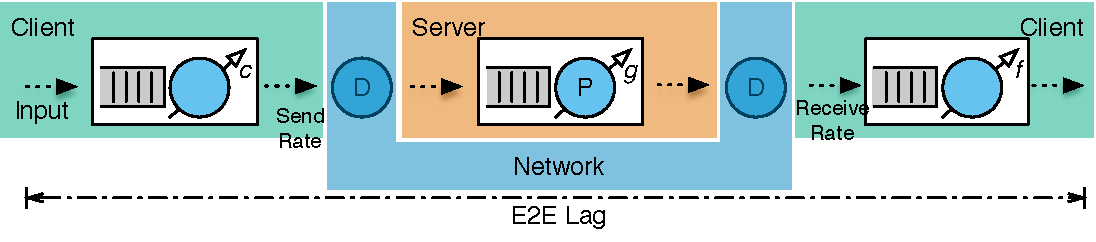
\includegraphics[width=1.0\textwidth]{images/e2e-lag-model.pdf}
	\caption{End-to-end lag model used as basis for this investigation. Several processes are assumed to be clocked, denoted by the diagonal arrows.}
\label{fig:e2e-lag-model}
\end{figure*}

In any video game a multitude of cogs is working in unison to transform a player's inputs into meaningful actions inside the game world. A simplified depiction of the processes a player action must go through before finally being to able to be displayed in a multiplayer game with an authoritative server is given in Fig.~\ref{fig:e2e-lag-model}. 

Besides additional lag incurred through the input and output devices' hardware (i.e. in this case mouse,keyboard and monitor) --- which can on their own still be significant\footnote{See, e.g. the investigation of keyboard latency at \url{https://danluu.com/keyboard-latency/}, in some cases exceeding \SI{50}{\milli\second}.}. The components (and the corresponding terminology) investigated here are outlined in \cite{Metzger+2016}, and are 
%
\begin{itemize}
	\item the generation of the input events by the player,
	\item the command message send process (from the client to the server),
	\item the network round-trip time,
	\item the server's game state update rate (i.e. the so-called ``tick rate''),
	\item the server's update send rate (server to clients),
	\item the client's frame rate (and additionally other lag-inducing factors at the client).
\end{itemize}
%
It should be noted, that there are usually certain lag compensation techniques \cite{bernier2001latency} in place that can conceal parts of the lag from the player by speculatively displaying the player's action's results before being confirmed by the remote server. The specific measures that Overwatch takes have not yet been further examined.

For this experiment several regular matches (i.e. Overwatch's default mode with two teams of six players each) were played from the perspective of one player on one PC that can not maintain a stable frame rate of \SI{60}{\hertz} throughout the match. Packet traces of the game's incoming and outgoing encrypted UDP traffic were recorded on the same PC and are the basis for this examination. 

The code for models derived here as well as the refined lag simulation for this game is available in the public repository that hosts this paper.\footnote{\url{https://github.com/fmetzger/overwatch-lag-model}}
The following sections each examine one of individual behavioral components of the game, as shown in the overview in Fig.~\ref{fig:e2e-lag-model}.


\subsection{Command Messages}

% TODO: state the nature of this figure: it is a fringe case, no such behavior could be observed on a computer with sufficient resources (and thus stable \SI{60}{\hertz} frame rate)
\begin{figure}[t]
	\centering
	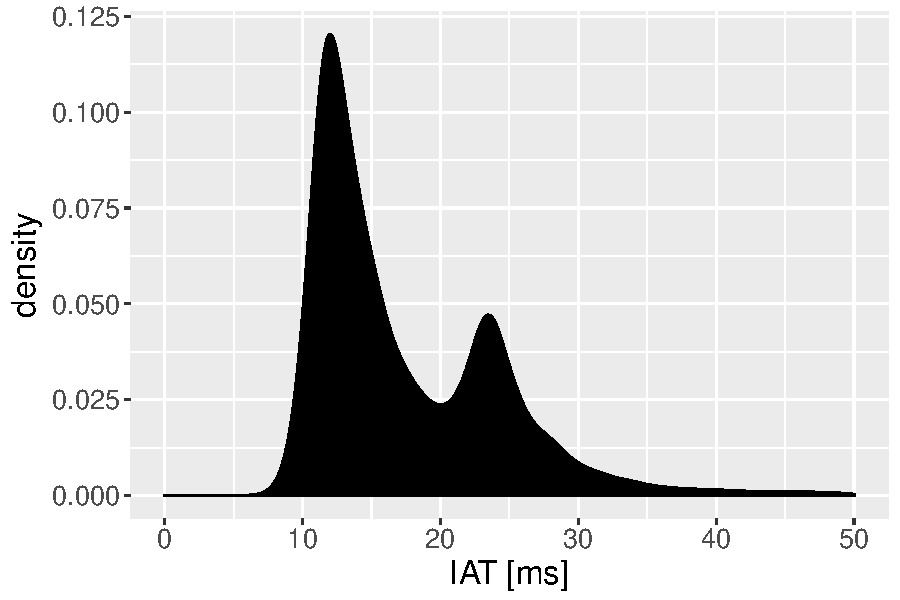
\includegraphics[width=1.0\columnwidth]{images/command-density.pdf}
	\caption{Continuous density plot of the command messages the client sends, showing a bimodal behavior instead of the expected single mode at \SI{16.7}{\milli\second}.}
\label{fig:command-density}
\end{figure}

The command messages are the messages the game clients sends to the server, containing all the player's inputs during that cycle. The developers of \textsc{Overwatch} advertise a tick rate (i.e. the frequency the server updates its game state) of \SI{60}{\hertz} (or an \gls{IAT} of about \SI{16.7}{\milli\second}. Therefore, one would assume that the game's transmission behavior targets the same values to incorporate all player decisions (i.e. inputs) in each update cycle and notify them of the resulting game state.

However, when looking at the density of the command message \glspl{IAT} in Fig.~\ref{fig:command-density}, actually two modes are revealed, one at around \SI{24}{\milli\second} (or a send rate of \SI{42}{\hertz}) and the other one at \SI{12}{\milli\second} (\SI{83}{\hertz}). Even though the overall mean \gls{IAT} is \SI{17.9}{\milli\second} and thus just slightly longer than required for the potentially targeted transmission rate of \SI{60}{\hertz}.

These modes are not distributed uniformly across the match but are rather separated into distinct transmission phases as the time series in Fig.~\ref{fig:command-timeseries} reveals. Here, the duration of the match can be divided into two alternating phases. The first phase reveals a (weak) third mode centered around \SI{16.7}{\milli\second}, i.e. the expected behavior of the game to send its inputs at a rate of \SI{60}{\hertz} to the server. But in the second phase, the game sends with both the \glspl{IAT} observed in Fig.~\ref{fig:command-density} at a ratio of about four to one in favor of the \SI{12}{\milli\second} intervals. The exact reason for this behavior is, as of yet, unknown, but could possibly be attributed to the resource constrained nature of the experiment. This bimodal behavior could not be observed on a second, sufficiently dimensioned, PC.

In order to model this behavior, the trace was split at those phases and each phase modeled separately. The \SI{60}{\hertz} phases were fitted to a Gamma distribution with $\Gamma(\alpha = 4.437922, \beta = 208.366)$, the second phases were mixed by a Gamma distribution $\Gamma(\alpha = 49.32119, \beta = 3970.154)$ for the \SI{83}{\hertz} portion and a Normal distribution $\mathcal{N}(\mu = 0.02359103, \sigma = 0.001369922)$ for \SI{42}{\hertz}). Finally, the phase lengths are giving by a set of two Normal distributions. $\mathcal{N}(\mu = 28.85714, \sigma = 1.216385)$ models the length of the unimodal \SI{60}{\hertz} phase, and $\mathcal{N}(\mu = 40.83333, \sigma = 2.054805)$ gives the length of the bimodal phase. A random sample generated with this model is depicted in the left panel of Fig.~\ref{fig:command-timeseries}.


\begin{figure}[t]
	\centering
	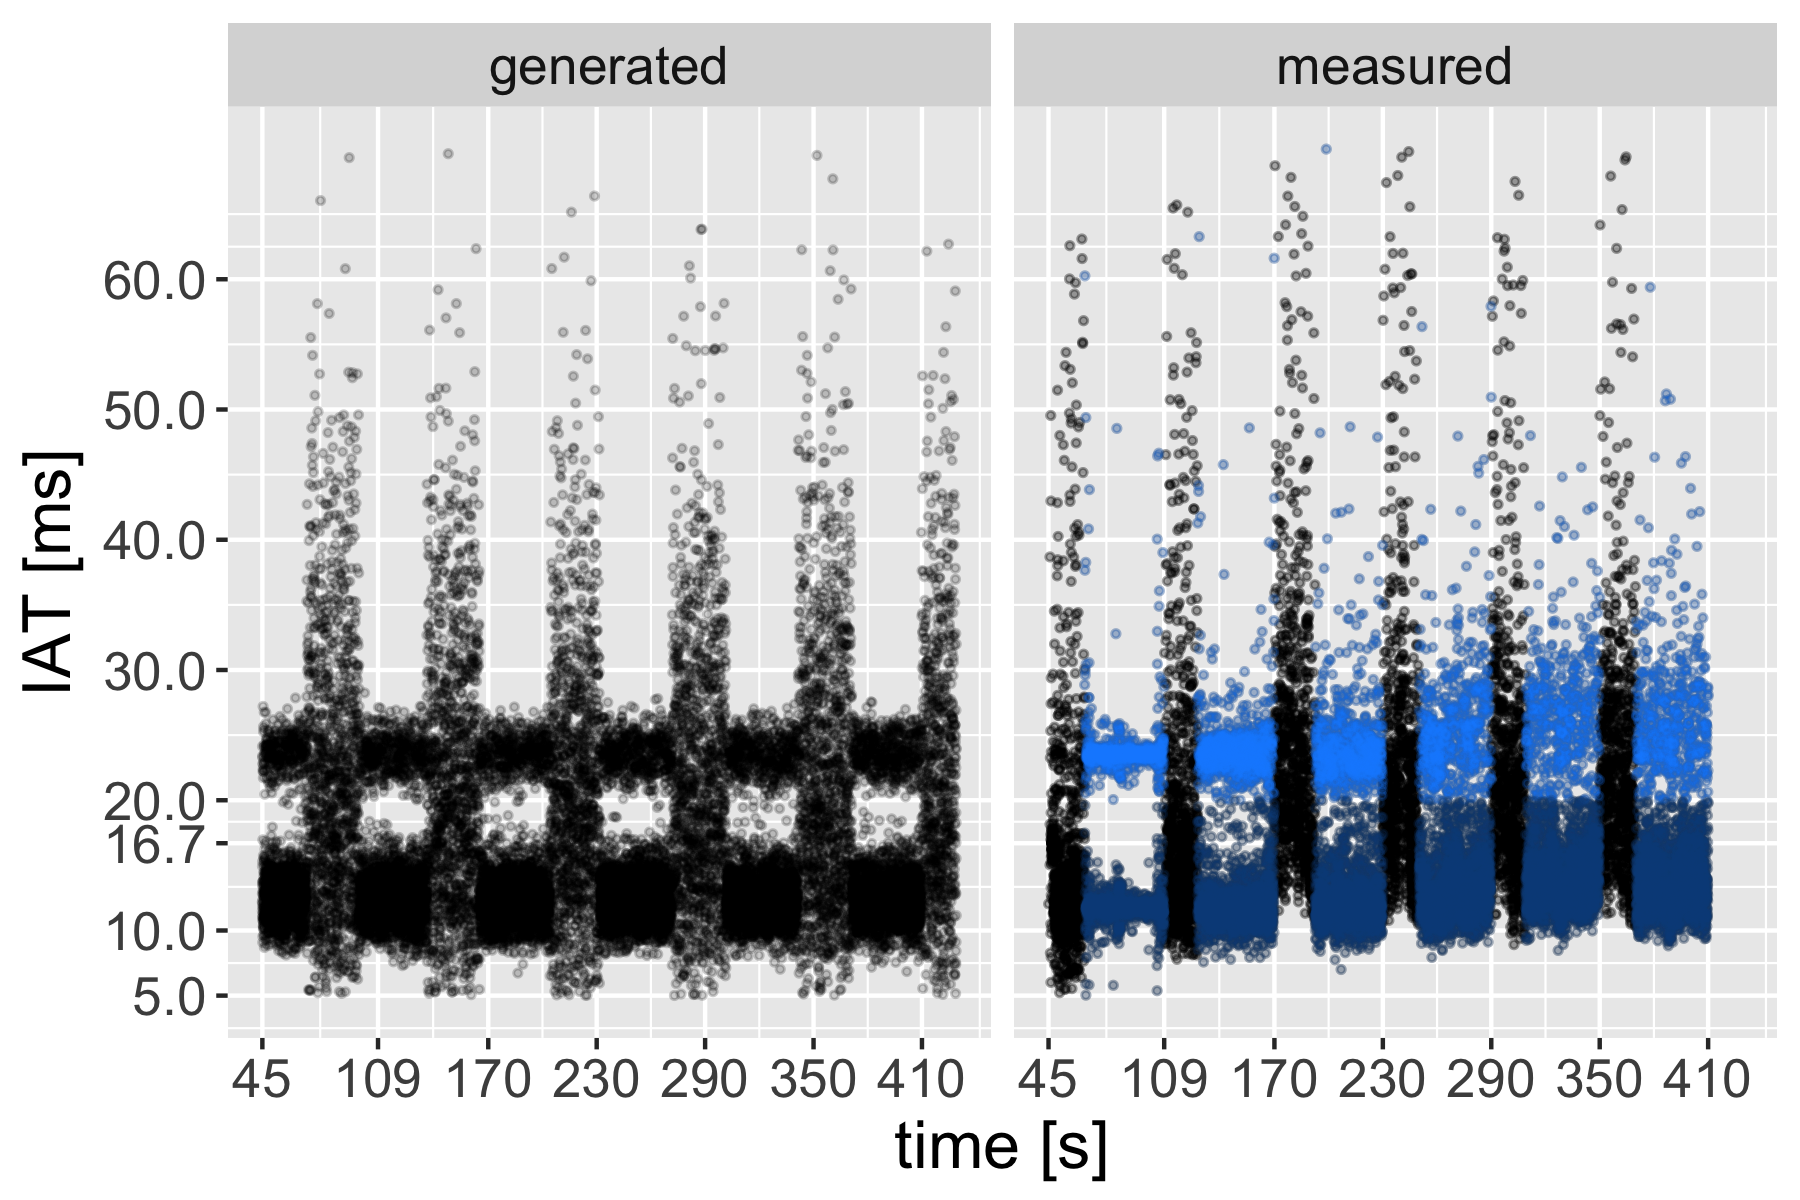
\includegraphics[width=1.0\columnwidth]{images/command-ts-annotated.png}
	\caption{Time series of the client-sent command messages both measured in the experiment as well as generated from the model. The different phases are highlighted in different colors.}
\label{fig:command-timeseries}
\end{figure}



\subsection{Game State Update Messages}

	\begin{figure}[t]
		\centering
		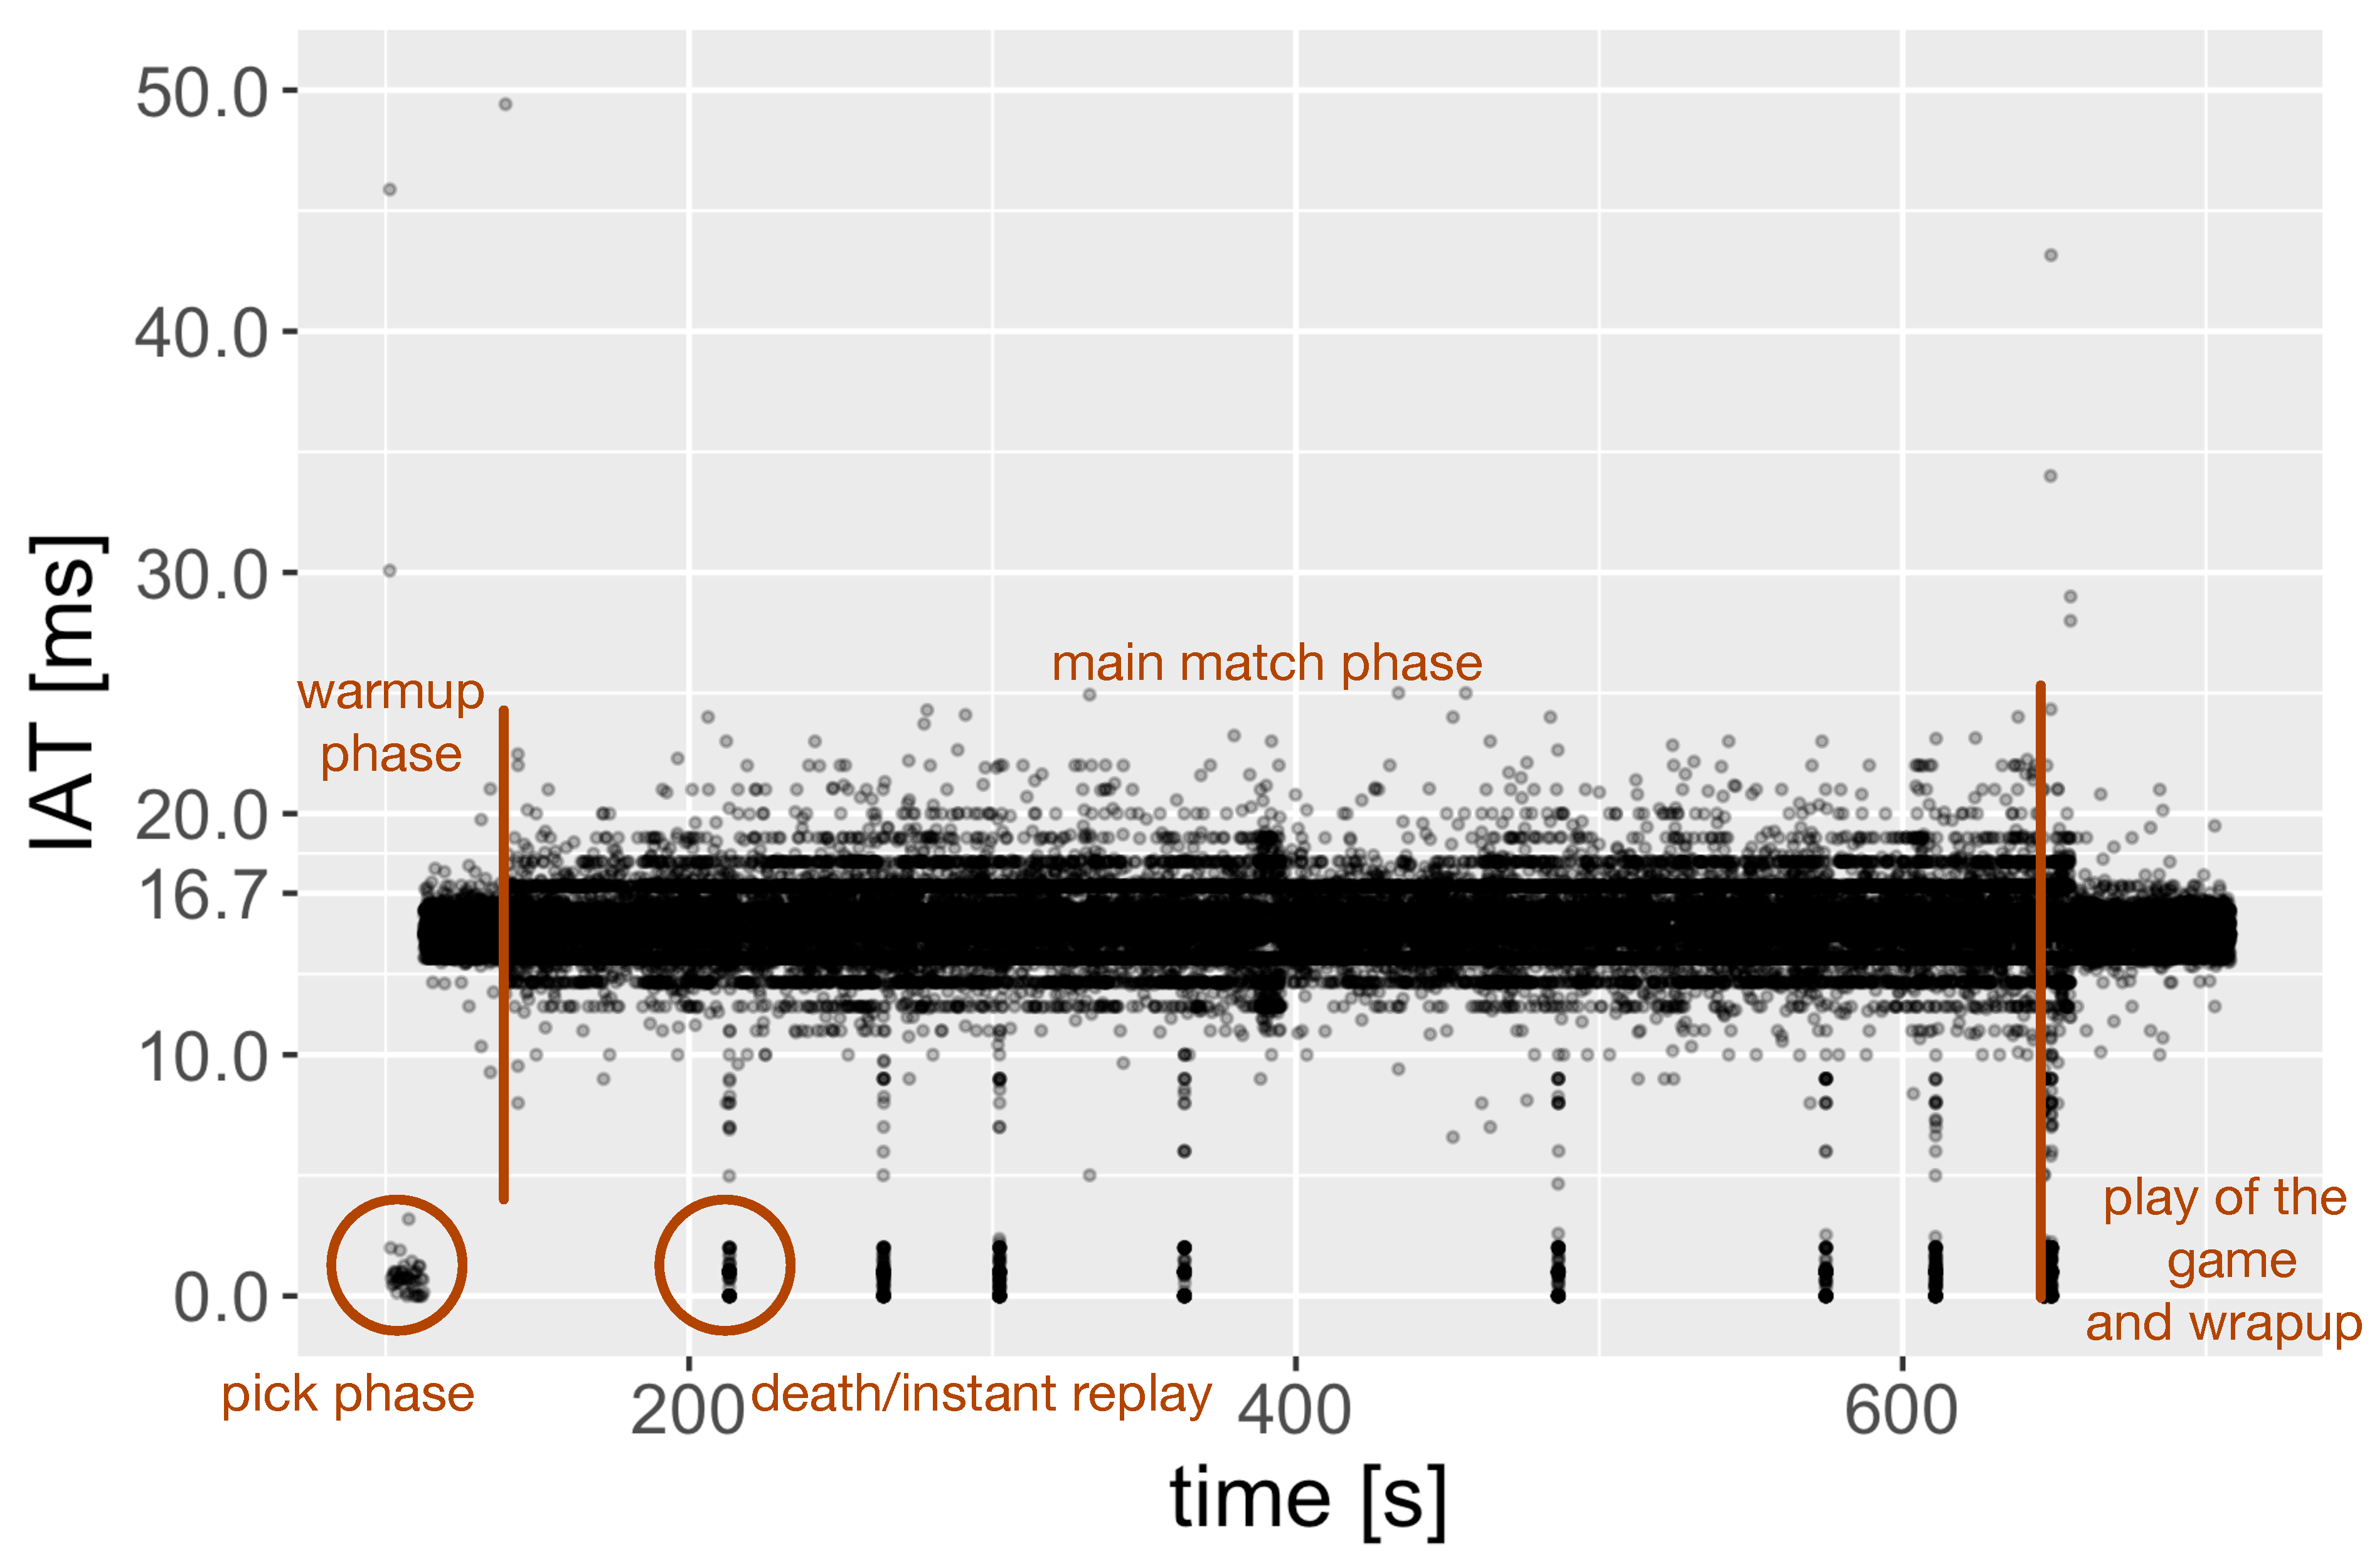
\includegraphics[width=1.0\columnwidth]{images/update-ts-annotated.pdf}
		\caption{Time series of the received game state update messages. The game phases and non-interactive ``kill cam'' events are annotated.}
	\label{fig:update-timeseries}
	\end{figure}

	\begin{figure}[t]
		\centering
		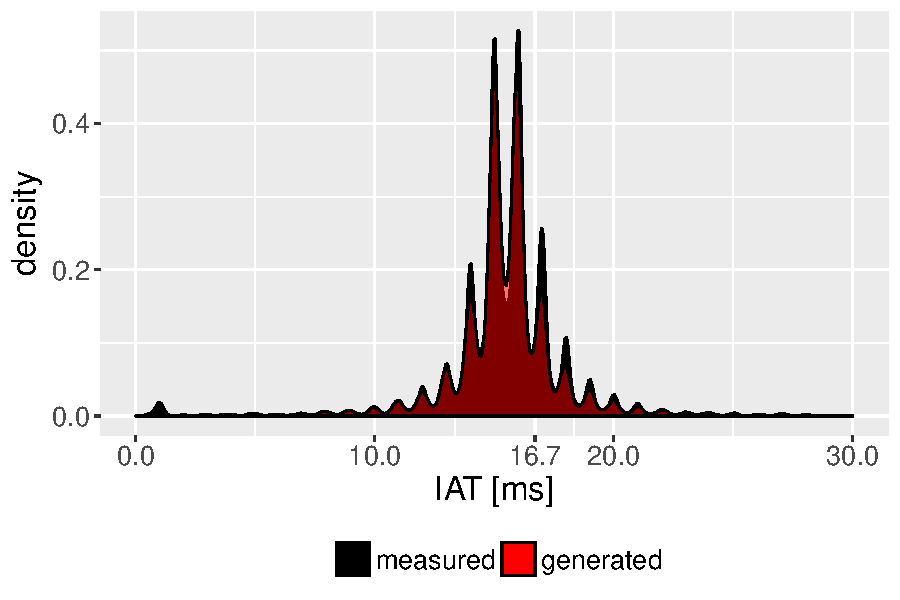
\includegraphics[width=1.0\columnwidth]{images/update-density.pdf}
		\caption{Density plot of both the measured and the fitted game state update messages received by the client.}
	\label{fig:update-density}
	\end{figure}

	The next lag component is the distribution of the game state update messages that the game server sends periodically to each connected game client. Ideally, such an update should be send immediately after every game simulation ``tick''. A time series of the client's packet reception \glspl{IAT} of one match is depicted in Fig.~\ref{fig:update-timeseries}. There are a few properties of note here, that clearly indicate that the server's messaging behavior depends on the game state even though the tick rate targets a rate of \SI{60}{\hertz}. 

	The first block of very short \glspl{IAT} directly maps to the pick phase of \textsc{Overwatch}, where each player picks the hero (or class) she is going to play during this match. The next, short phase (visible by less spread in the samples) is the warmup phase, where both teams can not yet leave their respective starting areas and thus no meaningful action can occur. Only after this phase the actual game starts and the spread of the \gls{IAT} increases, possibly hinting at increased load at the server side. Similar the final phase of less sample spread depicts the game after the match has ended and the players see match statistics as well as a replay of a noteworthy event in the match (the ``Play of the Game'').

	Every now and then the data exposes a quick burst of data in short intervals (i.e. the vertical bars in Fig.~\ref{fig:update-timeseries}). This directly correlates to the so-called ``kill cam''. When the player dies during the match, and before she respawns, she is shown a quick replay of the event from the perspective of the shooter. Thus, this replay data needs to be transferred to the player first. This feature can also be turned off, eliminating the burst of data alongside.	The reason for the grouping on the vertical axis into distinctly visible horizontal bars is not entirely clear yet, but is not necessarily present on each client PC. A quick check with the game running on another computer did not exhibit this behavior. Nonetheless, it is present here and certainly influences the \gls{E2E} lag and therefore should be considered in the model.

	Due to this oscillating behavior (cf. the density plot in Fig.~\ref{fig:update-density}) the update messaging process could best be modeled with a Cauchy distribution as base, modulated with a sine function. This yields
	%
	\begin{equation*}
		f_{rcv}(x) = \frac{0.7\sin(171.6 +3120x)^4 + 0.2}{0.9848153} f(x; x_0; \gamma)^{1.17} 
	\end{equation*}
	%
	for the density, with location $x_0 = 0.0155$ and scale $\gamma = 0.0011$ for the Cauchy distribution. It should be noted that this model is only applicable for the game's main phase and excludes the ``kill cam''-events as well. Those are either not relevant to the outcome of the match (warmup phase and post-match statistics) or are even entirely non-interactive for the player.



\subsection{Input Events}

Another component is the distribution of the actual input events that the player generates with her input devices. The original simulation in \cite{Metzger+2016} just assumed an exponential distribution with a rate that might not be entirely realistic for an actual game. Therefore, for \textsc{Overwatch} the inputs were recorded and a rate parameter for the exponential distribution was derived as a compound of button strokes and mouse movements ($\lambda = 102.1824$).


\subsection{Network Delay}

Finally, the network delay must also be considered. But due to the high reliability of servers and the matchmaking that should place the player on to a server in the player's vicinity, the delay to the server should be low and stable. In a separate RTT measurement to the game server's IP address found in the investigated matches the RTT was about \SI{34}{\milli\second}. This is used as a constant network delay component in the simulation. The low variance of the measured RTT does not justify a more complex distribution here.


%!TEX root = paper.tex
%%%%%%%%%%%%%%%%%%%%%%%%%%%%%%%%%%%%%%%%%%%%%%%%%%%%%%%%%%%%%%%%%%%%%%%%%%%%%%%%
\section{Overwatch Lag Simulation}
\label{sec:simulation}

\begin{figure}
	\centering
	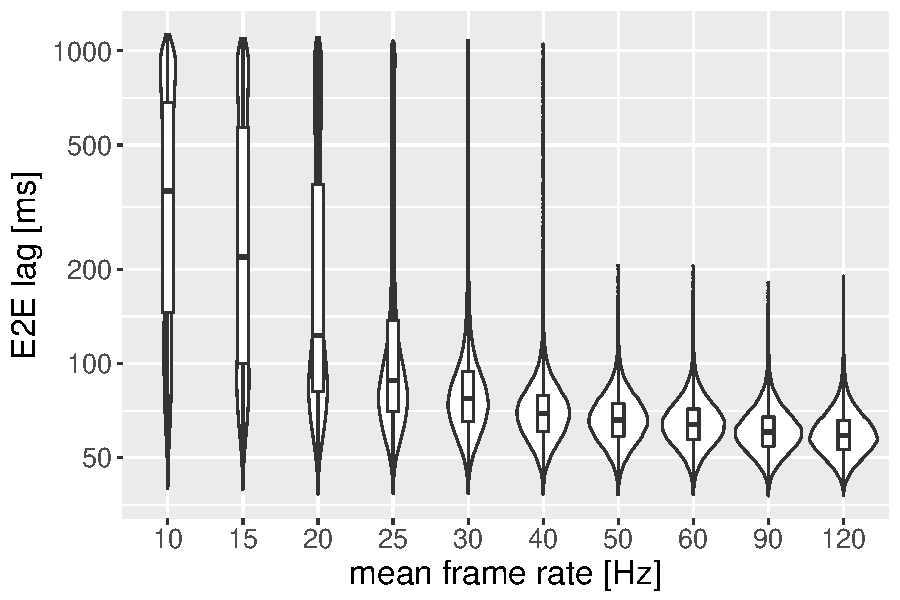
\includegraphics[width=1.0\columnwidth]{images/lagsim.pdf}
	\caption{\acrshort{E2E} lag results of a frame rate study using the \textsc{Overwatch} simulation. The denoted frame rates are the mean of the normal distribution.}
\label{fig:lagsim}
\end{figure}

% TODO: - Interpretation of Figure 5: what happens between 40 and 50 Hz (when the maximal E2E lag suddenly decreases from >1 s to >200 ms)? Why such an abrupt change?
% TODO: Why is there such a spread in the second phase? --- Answer we honestly do not know, but might be attributed to internal game behavior

Now that all client-observable parameters have been examined, a simulation study is performed on the effects of the game's frame rate. This the only direct game parameter that the player can influence through the game's setting or through more capable hardware that influences the lag. But, since it is often tricky to maintain a stable frame rate in such resource constrained environments, the frame rate in this simulation is modeled as a normal distribution instead of a fixed value. This should account for the variations in the frame times (the time between two consecutive frames). Investigated here were frame rates between \SI{10}{\hertz} and \SI{120}{\hertz}. The minimum value might occur in high stress situations when resource are severely constrained, and the maximum value representing what can be achieved with modern PC hardware and monitors. All other simulation parameters are derived from the models in the previous section or left as-is in the base simulation. 

The results are depicted in Fig.~\ref{fig:lagsim}. Starting at about \SI{50}{\hertz} the \gls{E2E} lag reduction sees diminishing returns especially towards its outliers, which can exceed a lag of over a second below \SI{50}{\hertz}. This correlates quite well with the generally accepted notion that (especially) online first person shooters require at least \SI{60}{\hertz} for an enjoyable experience. In praxis, only \SI{30}{\hertz}, \SI{60}{\hertz} or higher frame rates will be targeted, due to otherwise occurring interactions with the monitor's refresh rate, which results in either screen tearing or an unstable \gls{IAT} of the rendered frames.

%!TEX root = paper.tex
%%%%%%%%%%%%%%%%%%%%%%%%%%%%%%%%%%%%%%%%%%%%%%%%%%%%%%%%%%%%%%%%%%%%%%%%%%%%%%%%
\section{Conclusion}
\label{sec:conclusion}

This lag model for \textsc{Overwatch} is highly customized and unfortunately not a one-size-fits-all solution for every game. But it still gives much needed insights into the dynamics of video games and the deviations from the theoretical properties that are actually happening in praxis. With that being said, even the refined simulation clearly demonstrates the strong influence of the game's frame rate and input and messaging processes investigated here on the \gls{E2E} lag, despite operating under near-ideal network conditions.


\printbibliography

\balance

\end{document}
